\documentclass[table]{beamer}
%[]中可以使用draft、handout、screen、transparency、trancompress、compress等参数

%指定beamer的模式与主题
\mode<presentation>
{
  \usetheme{Madrid}
%\usetheme{Boadilla}
%\usecolortheme{default}
%\usecolortheme{orchid}
%\usecolortheme{whale}
%\usefonttheme{professionalfonts}
}

%\usetheme{Madrid}
%这里还可以选择别的主题:Bergen, Boadilla, Madrid, AnnArbor, CambridgeUS, Pittsburgh, Rochester, Warsaw, ...
%有导航栏的Antibes, JuanLesPins, Montpellier, ...
%有内容的Berkeley, PaloAlto, Goettingen, Marburg, Hannover, ...
%有最小导航栏的Berlin, Ilmenau, Dresden, Darmstadt, Frankfurt, Singapore, Szeged, ...
%有章和节表单的Copenhagen, Luebeck, Malmoe, Warsaw, ...

%\usecolortheme{default}
%设置内部颜色主题(这些主题一般改变block里的颜色);这个主题一般选择动物来命名
%这里还可以选择别的颜色主题,如默认的和有特别目的的颜色主题default,structure,sidebartab,全颜色主题albatross,beetle,crane,dove,fly,seagull,wolverine,beaver

%\usecolortheme{orchid}
%设置外部颜色主题(这些主题一般改变title里的颜色);这个主题一般选择植物来命名
%这里还可以选择别的颜色主题,如默认的和有特别目的的颜色主题lily,orchid,rose

%\usecolortheme{whale}
%设置字体主题;这个主题一般选择海洋动物来命名
%这里还可以选择别的颜色主题,如默认的和有特别目的的颜色主题whale,seahorse,dolphin

%\usefonttheme{professionalfonts}
%类似的还可以定义structurebold,structuresmallcapsserif,professionalfonts


% 控制 beamer 的风格,可以根据自己的爱好修改
%\usepackage{beamerthemesplit} %使用 split 风格
%\usepackage{beamerthemeshadow} %使用 shadow 风格
%\usepackage[width=2cm,dark,tab]{beamerthemesidebar}

%插入音标
\usepackage{tipa}
\AtBeginDocument{
  \renewcommand\textipa{\fontencoding{T3}\selectfont}
}
\AtBeginDocument{
  \renewcommand\textipa[2][r]{{\fontfamily{cm#1}\tipaencoding #2}}
}
\renewenvironment{IPA}[1][r]
 {\fontfamily{cm#1}\tipaencoding}
 {}

% 设定英文字体
%\usepackage{fontspec}
\usepackage[no-math]{fontspec}
\setmainfont{Times New Roman}
\setsansfont{Arial}
\setmonofont{Courier New}

% 设定中文字体
\usepackage[BoldFont,SlantFont,CJKchecksingle,CJKnumber]{xeCJK}
%\setCJKmainfont[BoldFont={Adobe Heiti Std},ItalicFont={Adobe Kaiti Std}]{Adobe Song Std}
\setCJKmainfont[BoldFont={Adobe Heiti Std},ItalicFont={Adobe Kaiti Std}]{WenQuanYi Micro Hei}
\setCJKsansfont{Adobe Heiti Std}
\setCJKmonofont{Adobe Fangsong Std}
\punctstyle{hangmobanjiao}

\defaultfontfeatures{Mapping=tex-text}
\usepackage{xunicode}
\usepackage{xltxtra}

\XeTeXlinebreaklocale "zh"
\XeTeXlinebreakskip = 0pt plus 1pt minus 0.1pt

\usepackage{setspace}
\usepackage{colortbl,xcolor}
\usepackage{hyperref}
%\hypersetup{xetex,bookmarksnumbered=true,bookmarksopen=true,pdfborder=1,breaklinks,colorlinks,linkcolor=blue,filecolor=black,urlcolor=cyan,citecolor=green}
\hypersetup{xetex,bookmarksnumbered=true,bookmarksopen=true,pdfborder=1,breaklinks,colorlinks,linkcolor=cyan,filecolor=black,urlcolor=blue,citecolor=green}

% 插入图片
\usepackage{graphicx}
\graphicspath{{figures/}}
% 图文混排
\usepackage{picins}
\usepackage{floatflt}

% 可能用到的包
\usepackage{amsmath,amssymb}
%插入多媒体
%\usepackage{media9}
%\usepackage{movie15}
\usepackage{multimedia}
\usepackage{multicol}
\usepackage{multirow}

% 定义一些自选的模板,包括背景、图标、导航条和页脚等,修改要慎重
% 设置背景渐变由10%的红变成10%的结构颜色
%\beamertemplateshadingbackground{red!10}{structure!10}
%\beamertemplatesolidbackgroundcolor{white!90!blue}
% 使所有隐藏的文本完全透明、动态,而且动态的范围很小
\beamertemplatetransparentcovereddynamic
% 使itemize环境中变成小球,这是一种视觉效果
\beamertemplateballitem
% 为所有已编号的部分设置一个章节目录,并且编号显示成小球
\beamertemplatenumberedballsectiontoc
% 将每一页的要素的要素名设成加粗字体
\beamertemplateboldpartpage

% item逐步显示时,使已经出现的item、正在显示的item、将要出现的item呈现不同颜色
\def\hilite<#1>{
 \temporal<#1>{\color{gray}}{\color{blue}}
    {\color{blue!25}}
}

\renewcommand{\today}{\number\year 年 \number\month 月 \number\day 日}

%五角星
\usepackage{MnSymbol}

%去除图表标题中的figure等
\usepackage{caption}
\captionsetup{labelformat=empty,labelsep=none}

\usepackage{tabu}
\usepackage{multirow}
%表格自动换行
\usepackage{tabularx} 

% 千分号
%\usepackage{textcomp}

%罗马数字
\makeatletter
\newcommand{\rmnum}[1]{\romannumeral #1}
\newcommand{\Rmnum}[1]{\expandafter\@slowromancap\romannumeral #1@}
\makeatother

%分栏
\usepackage{multicol}

%\usepackage{enumitem}
%\usepackage{enumerate}

%键盘
\usepackage{keystroke}

%插入源代码
\usepackage{listings}
\lstset{
  language=bash,                  % 程序语言名称:TeX, Perl, R, sh, bash, Awk
  basicstyle=\normalsize\tt,      %\tt指monospace字体族,程序源代码使用此族字体表示更加美观
  numbers=left,                   % 行号位置(左侧)
  numberstyle=\small,             % 行号字体的字号
  stepnumber=1,                   % 行号的显示步长
  numbersep=5pt,                  % 行号与代码间距
  backgroundcolor=\color{white},  % 背景色;需要 \usepackage{color}
  showspaces=false,               % 不显示空格
  showstringspaces=false,         % 不显示代码字符串中的空格标记
  showtabs=false,                 % 不显示 TAB
  tabsize=4, 
  frame=shadowbox,                % 把代码用带有阴影的框圈起来
  captionpos=b,                   % 标题位置
  breaklines=true,                % 对过长的代码自动断行
  breakatwhitespace=false,        % 断行只在空格处
  extendedchars=false,            % 解决代码跨页时,章节标题,页眉等汉字不显示的问题
  %escapeinside={\%*}{*},         % 跳脱字符,添加注释,暂时离开 listings 
  %escapeinside=``,
  commentstyle=\color{red!50!green!50!blue!50}\tt,  %浅灰色的注释
  rulesepcolor=\color{red!20!green!20!blue!20},     %代码块边框为淡青色
  keywordstyle=\color{blue!70}\bfseries\tt,         %代码关键字的颜色为蓝色,粗体
  identifierstyle=\tt,
  stringstyle=\tt,                % 代码字符串的特殊格式
  keepspaces=true,
  breakindent=1em,
  %breakindent=22pt,
  %breakindent=4em,
  breakautoindent=true,
  flexiblecolumns=true,
  aboveskip=1em,                  %代码块边框
  xleftmargin=2em,
  xrightmargin=2em
}

%\setbeamercolor{alerted text}{fg=magenta}
\setbeamercolor{bgcolor}{fg=yellow,bg=cyan}
%\setbeamercolor{itemize/enumerate body}{fg=green}

\begin{document}

%\includeonlyframes{current}

\logo{
\includegraphics[height=0.08\textwidth]{tijmu.png}}

% 在每个Section前都会加入的Frame
\AtBeginSection[]
{
  \begin{frame}<beamer>
    %\frametitle{Outline}
    \frametitle{教学提纲}
    \setcounter{tocdepth}{3}
    \begin{multicols}{2}
      \tableofcontents[currentsection,currentsubsection]
      %\tableofcontents[currentsection]
    \end{multicols}
  \end{frame}
}
% 在每个Subsection前都会加入的Frame
\AtBeginSubsection[]
{
  \begin{frame}<beamer>
%%\begin{frame}<handout:0>
%% handout:0 表示只在手稿中出现
    \frametitle{教学提纲}
    \setcounter{tocdepth}{3}
    \begin{multicols}{2}
    \tableofcontents[currentsection,currentsubsection]
    \end{multicols}
%% 显示在目录中加亮的当前章节
  \end{frame}
}

% 为当前幻灯片设置背景
%{
%\usebackgroundtemplate{
%\vbox to \paperheight{\vfil\hbox to
%\paperwidth{\hfil
\includegraphics[width=2in]{tijmu_charcoal.png}\hfil}\vfil}
%}
\begin{frame}[plain]
  \begin{center}
    {\Huge Linux系统概论\\}
    \vspace{1cm}
    {\LARGE 天津医科大学\\}
    %\vspace{0.2cm}
    {\LARGE 生物医学工程与技术学院\\}
    \vspace{1cm}
    {\large 2017-2018学年下学期(春)\\ 2016级生信班}
  \end{center}
\end{frame}
%}



%\includeonlyframes{current}

\title[用户和组]{第二章\quad 用户和组}
\author[Yixf]{伊现富(Yi Xianfu)}
\institute[TIJMU]{天津医科大学(TIJMU)\\ 生物医学工程与技术学院}
\date{2018年5月}


\begin{frame}
  \titlepage
\end{frame}

\begin{frame}[plain,label=current]
  \frametitle{教学提纲}
  \setcounter{tocdepth}{3}
  \begin{multicols}{2}
    \tableofcontents
  \end{multicols}
\end{frame}

\section{引言}
\begin{frame}
  \frametitle{用户和组 | 引言 | 通行证}
  \begin{figure}
    \centering
    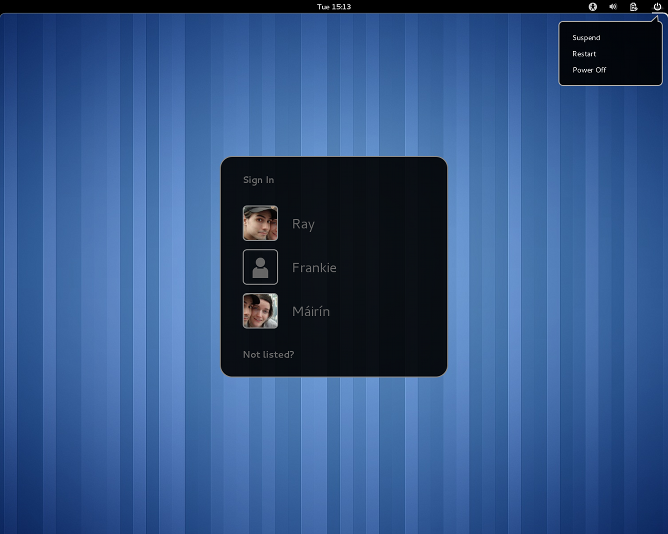
\includegraphics[width=9cm]{c2.login.png}
  \end{figure}
\end{frame}

\section{账户}
\subsection{三类账户}
\begin{frame}
  \frametitle{用户和组 | 账户 | \alert{三大类}}
  \begin{enumerate}
    \item<1-> 根账户(根用户/超级用户账户,root,UID=0)
      \begin{itemize}
        \item<4-> 不受任何限制,能够进行任何操作,包括自我毁灭
        \item<5-> 谨慎使用,仅在必要且用于最重要的任务时使用
      \end{itemize}
    \item<2-> 系统账户(伪用户,UID:1-499/999;CentOS/Ubuntu)
      \begin{itemize}
        \item<6-> 与系统和程序服务相关
	  \begin{itemize}
	    \item bin、daemon、shutdown、halt等,任何Linux系统默认都有这些伪用户
	    \item mail、news、games、apache、ftp、mysql及sshd等,与Linux系统的进程相关
            \item 通常不需要或无法登录系统
            \item 可以没有家目录
	  \end{itemize}
        \item<6-> 由操作系统在安装过程中提供或由软件制造商提供
        \item<6-> 对系统特定组件进行操作,协助用户所需的服务或程序
        \item<7-> 不要轻易修改,否则可能会给系统带来不良影响
      \end{itemize}
    \item<3-> 用户账户(普通用户账户,UID:500/1000-60000;CentOS/Ubuntu)
      \begin{itemize}
        \item<8-> 为用户和用户组提供对系统的交互式访问
        \item<8-> 对关键系统文件和目录的访问权限是有限的
      \end{itemize}
  \end{enumerate}
\end{frame}

\begin{frame}
  \frametitle{用户和组 | 账户 | 三大类 | 根账户}
  \begin{figure}
    \centering
    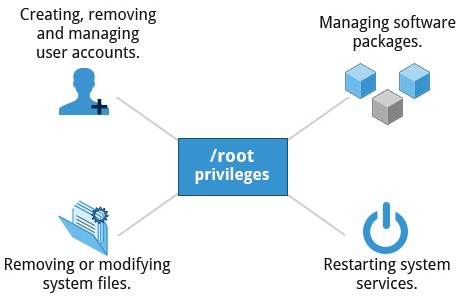
\includegraphics[width=10cm]{c2.root.jpg}
  \end{figure}
\end{frame}

\begin{frame}
  \frametitle{用户和组 | 账户 | 三大类 | 用户账户}
  \begin{figure}
    \centering
    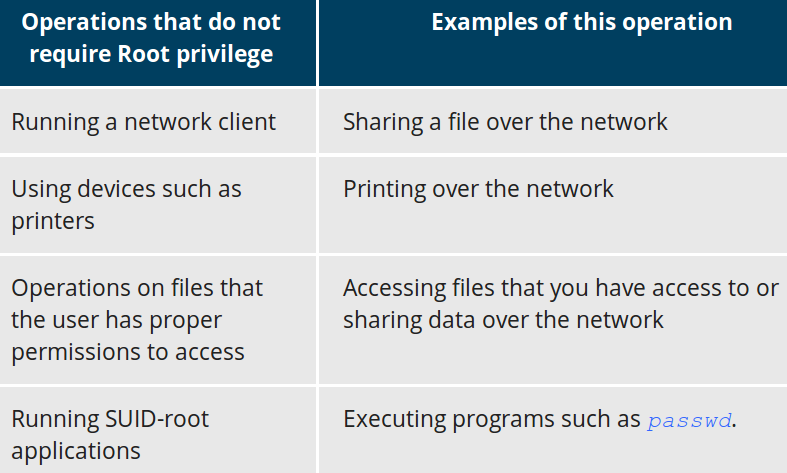
\includegraphics[width=11cm]{c2.user.png}
  \end{figure}
\end{frame}

\subsection{组账户}
\begin{frame}
  \frametitle{用户和组 | 账户 | 组账户}
  \begin{block}{组账户}
    \begin{itemize}
      \item 为了简化权限管理,将多个账户集中在一起形成一个组
      \item 一个组可以包括多个账户,一个账户至少属于一个组
      \item 同一组的用户享有该组共有的权限
    \end{itemize}
  \end{block}
  \pause
  \begin{block}{权限管理中的\alert{三类用户}}
    \begin{itemize}
      \item 用户:文件的所有者
      \item 组:指派给文件的组
      \item 其他:系统中既不是所有者也不属于组的用户
    \end{itemize}
  \end{block}
\end{frame}

\section{用户管理文件}
\subsection{配置文件}
\begin{frame}
  \frametitle{用户和组 | \alert{配置文件}}
  \begin{table}
    \centering
    \rowcolors[]{1}{blue!20}{blue!10}
    \begin{tabularx}{\textwidth}{cXX}
      \hline
      \rowcolor{blue!50}文件 & 用途 & 说明\\
      \hline
      /etc/passwd & 用户信息文件,为系统识别已授权的用户 & 任何用户都可以查看,只有根用户才能修改\\
      /etc/shadow & 密码文件,保存相应账户加密后的口令 & 普通用户无法查看,根用户能读取但不能直接编辑\\
      /etc/group & 用户组文件,存放组账户的信息 & 同/etc/passwd\\
      /etc/gshadow & 用户组密码文件,保存相应组加密后的口令 & 同/etc/shadow\\
      \hline
    \end{tabularx}
  \end{table}
\end{frame}

\begin{frame}
  \frametitle{用户和组 | 配置文件 | 其他}
  \begin{table}
    \centering
    \rowcolors[]{1}{blue!20}{blue!10}
    \begin{tabularx}{0.6\textwidth}{cX}
      \hline
      \rowcolor{blue!50}文件 & 用途\\
      \hline
      /etc/login.defs & 用户配置文件\\
      /etc/default/useradd & 用户配置文件\\
      /etc/skel & 新用户信息文件\\
      /etc/issue & 登录信息\\
      \hline
    \end{tabularx}
  \end{table}
\end{frame}

\begin{frame}
  \frametitle{用户和组 | 配置文件 | 用户}
  \begin{figure}
    \centering
    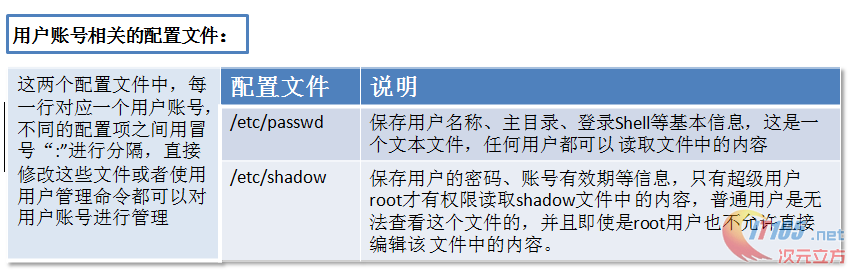
\includegraphics[width=12cm]{c2.user.file.png}
  \end{figure}
\end{frame}

\begin{frame}
  \frametitle{用户和组 | 配置文件 | 组}
  \begin{figure}
    \centering
    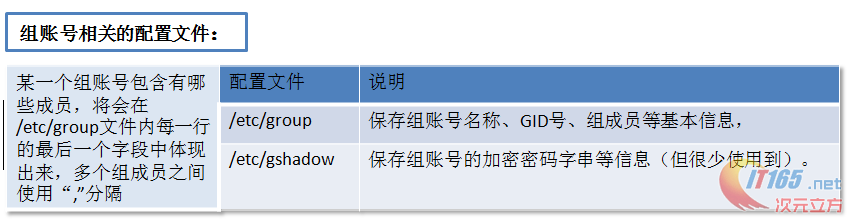
\includegraphics[width=12cm]{c2.group.file.png}
  \end{figure}
\end{frame}

\subsection{/etc/passwd}
\begin{frame}
  \frametitle{用户和组 | 配置文件 | /etc/passwd}
  \begin{figure}
    \centering
    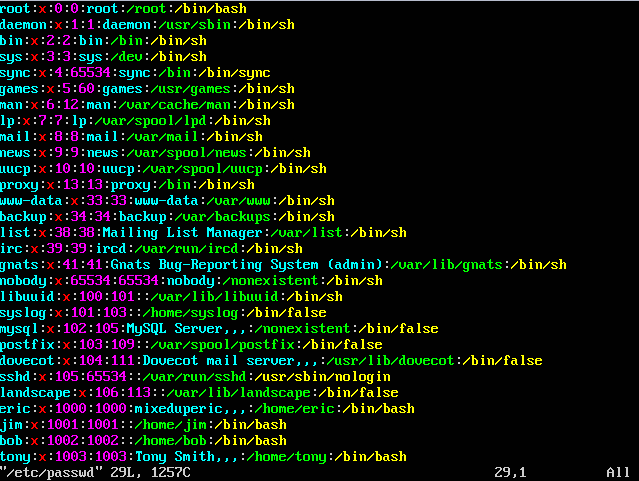
\includegraphics[width=10cm]{c2.passwd.png}
  \end{figure}
\end{frame}

\begin{frame}
  \frametitle{用户和组 | 配置文件 | /etc/passwd | \alert{7个字段}}
  \vspace{-0.5cm}
  \begin{figure}
    \centering
    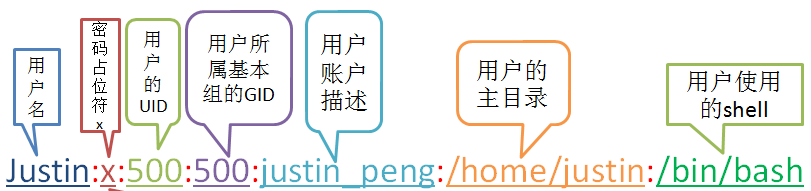
\includegraphics[width=10cm]{c2.passwd.fields.01.png}
  \end{figure}
  \pause
  \vspace{-0.5cm}
  \begin{table}
    \centering
    \rowcolors[]{1}{blue!20}{blue!10}
    \begin{tabularx}{\textwidth}{clX}
      \hline
      \rowcolor{blue!50}字段 & 含义 & 说明\\
      \hline
      1 & 用户名 & 用户登录系统时输入的账户;UID的字符串标记方式,方便阅读\\
      2 & 密码 & x,密码位,密码放在/etc/shadow中\\
      3 & UID & User ID,用户标识号\\
      4 & GID & Group ID,默认组标识号\\
      5 & 注释 & 账户的相关信息(全名、电话等)\\
      6 & 家目录 & 宿主目录,用户登录系统后默认所处的目录\\
      7 & 登录shell & 用户登录系统后默认所使用的shell\\
      \hline
    \end{tabularx}
  \end{table}
\end{frame}

\begin{frame}
  \frametitle{用户和组 | 配置文件 | /etc/passwd | 7个字段}
  \begin{figure}
    \centering
    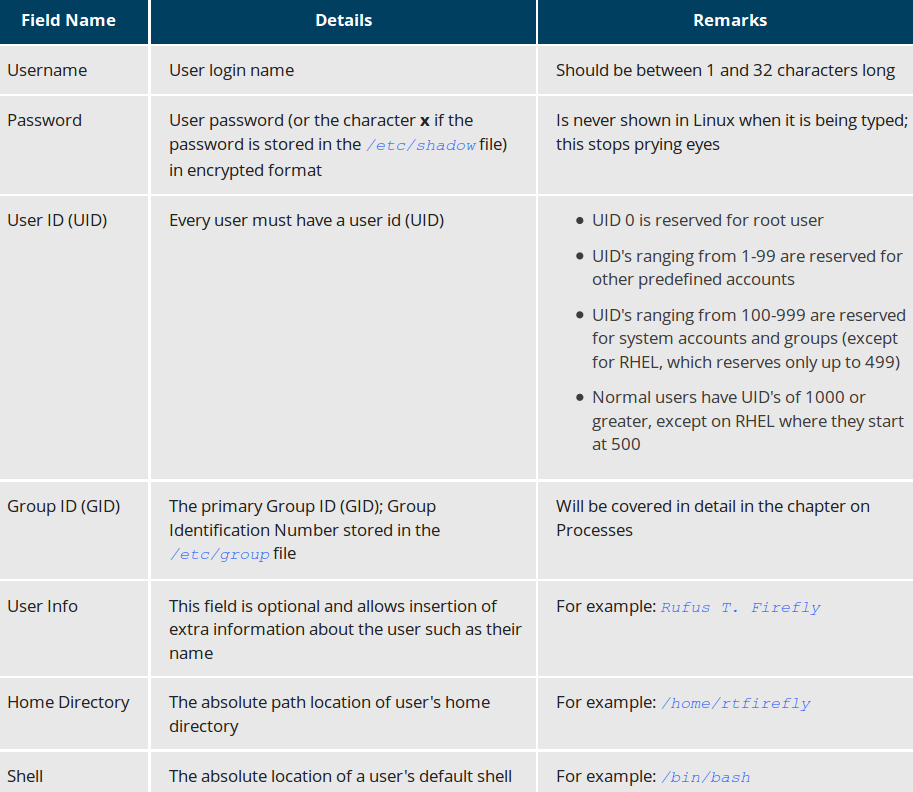
\includegraphics[width=11cm,height=7.5cm]{c2.passwd.fields.20.png}
  \end{figure}
\end{frame}

\begin{frame}
  \frametitle{用户和组 | 配置文件 | /etc/passwd | UID}
  \begin{figure}
    \centering
    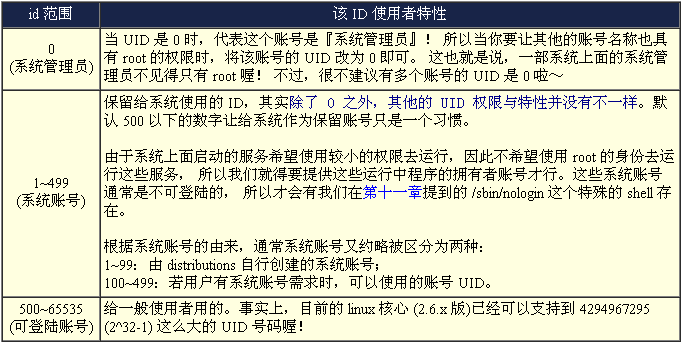
\includegraphics[width=12cm]{c2.uid.png}
  \end{figure}
\end{frame}

\begin{frame}
  \frametitle{用户和组 | 配置文件 | /etc/passwd | UID \& GID}
  \begin{figure}
    \centering
    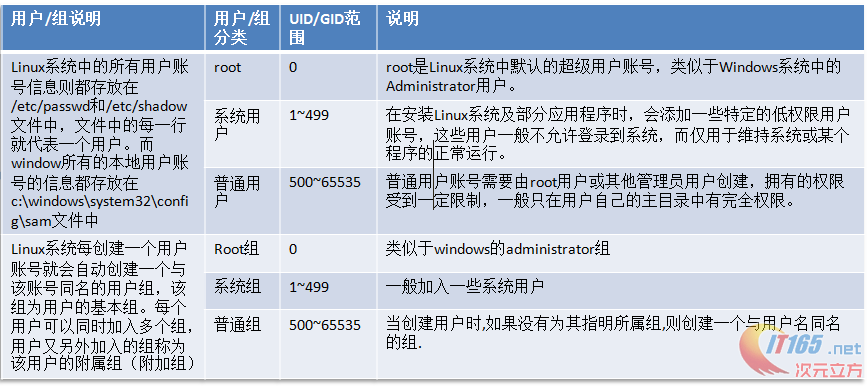
\includegraphics[width=12cm]{c2.uid.gid.png}
  \end{figure}
\end{frame}

\subsection{/etc/shadow}
\begin{frame}
  \frametitle{用户和组 | 配置文件 | /etc/shadow}
  \begin{figure}
    \centering
    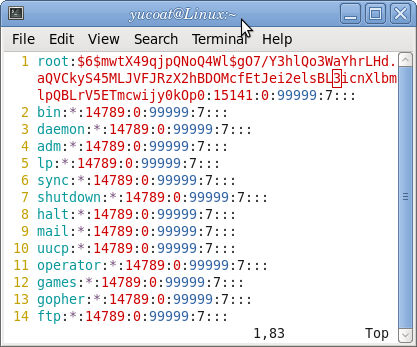
\includegraphics[width=9cm]{c2.shadow.jpg}
  \end{figure}
\end{frame}

\begin{frame}
  \frametitle{用户和组 | 配置文件 | /etc/shadow | 9个字段}
  \begin{figure}
    \centering
    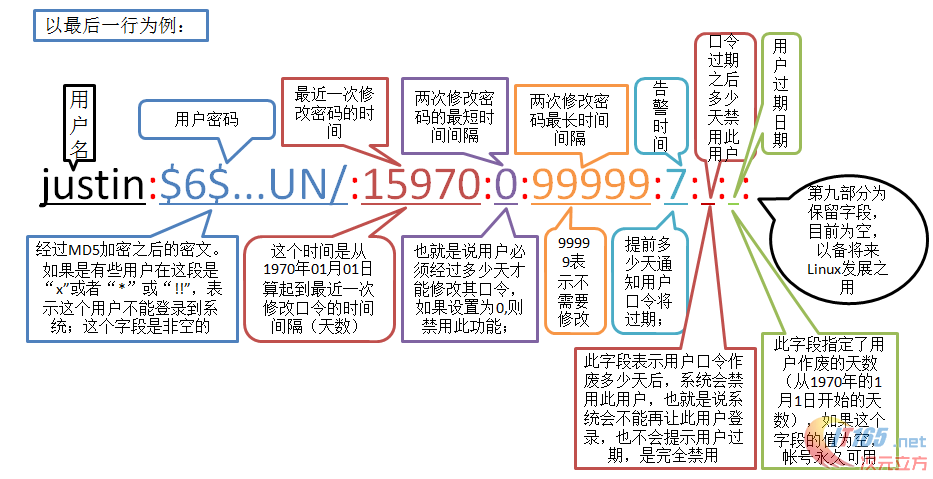
\includegraphics[width=12cm]{c2.shadow.fields.png}
  \end{figure}
\end{frame}

\begin{frame}
  \frametitle{用户和组 | 配置文件 | /etc/shadow | 9个字段}
  \begin{table}
    \centering
    \rowcolors[]{1}{blue!20}{blue!10}
    \begin{tabularx}{\textwidth}{clX}
      \hline
      \rowcolor{blue!50}字段 & 含义 & 说明\\
      \hline
      1 & 用户名 & 与/etc/passwd文件中的第一个字段相对应\\
      2 & 密码 & 加密后的密码\\
      3 & 最后一次修改密码的时间 & 上一次修改密码的日期与1970-01-01相距的天数\\
      4 & 两次修改密码的最短时间间隔 & 0表示禁用,随时可以修改密码\\
      5 & 两次修改密码的最长时间间隔 & 99999表示不需要修改密码\\
      6 & 告警时间 & 修改期限前N天通知用户密码将过期\\
      7 & 宽限时间 & 宽限期一过,账号将被完全禁用\\
      8 & 账号失效日期 & 从1970-01-01开始;为空时表示账号永久可用\\
      9 & 保留字段 & 以备将来使用\\
      \hline
    \end{tabularx}
  \end{table}
\end{frame}

\begin{frame}[fragile]
  \frametitle{用户和组 | 配置文件 | /etc/shadow | 9个字段 | 密码}
  \begin{enumerate}
    \item 奇奇怪怪的字符串:加密过的密码文件 
      \begin{itemize}
        \item 以\verb|$1$|起始:MD5加密
        \item 以\verb|$2a$|起始:Blowfish加密
        \item 以\verb|$2y$|起始:Blowfish(correct handling of 8-bit chars)加密
        \item 以\verb|$5$|起始:SHA-256加密
        \item 以\verb|$6$|起始:SHA-512加密
      \end{itemize}
    \item 星号\verb|*|,叹号\verb|!|,两个叹号\verb|!!|:\alert{帐号被锁定}
      \begin{itemize}
        \item 星号\verb|*|,或\verb|*LK*|:帐号被锁定
        \item 一个叹号\verb|!|,后跟加密的密码:有密码但被锁定,便于日后解锁
        \item 两个叹号\verb|!!|:未设置密码且被锁定;密码已经过期
      \end{itemize}
    \item 字段为空:没有密码
  \end{enumerate}
\end{frame}

\subsection{/etc/group}
\begin{frame}
  \frametitle{用户和组 | 配置文件 | /etc/group}
  \begin{figure}
    \centering
    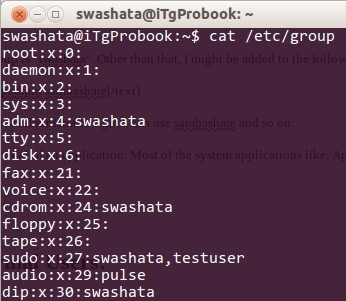
\includegraphics[width=8cm]{c2.group.jpg}
  \end{figure}
\end{frame}

\begin{frame}
  \frametitle{用户和组 | 配置文件 | /etc/group | \alert{4个字段}}
  \vspace{-0.3cm}
  \begin{figure}
    \centering
    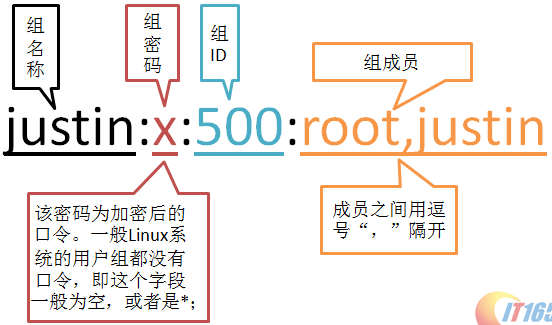
\includegraphics[width=8cm]{c2.group.fields.01.png}
  \end{figure}
  \pause
  \vspace{-0.5cm}
  \begin{table}
    \centering
    \rowcolors[]{1}{blue!20}{blue!10}
    \begin{tabularx}{\textwidth}{clX}
      \hline
      \rowcolor{blue!50}字段 & 含义 & 说明\\
      \hline
      1 & 组名 & 用户通过它来识别组\\
      2 & 组密码 & 空:没有组密码;x:密码位,密码放在/etc/gshadow中\\
      3 & GID & Group ID,标识系统中的组\\
      4 & 组成员 & 属于组的账户列表,账户之间用逗号隔开\\
      \hline
    \end{tabularx}
  \end{table}
\end{frame}

\subsection{/etc/gshadow}
\begin{frame}
  \frametitle{用户和组 | 配置文件 | /etc/gshadow}
  \begin{figure}
    \centering
    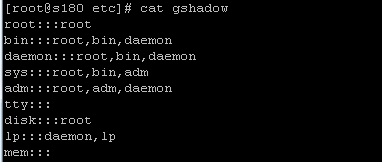
\includegraphics[width=10cm]{c2.gshadow.png}
  \end{figure}
\end{frame}

\begin{frame}
  \frametitle{用户和组 | 配置文件 | /etc/gshadow | 4个字段}
  \vspace{-0.3cm}
  \begin{figure}
    \centering
    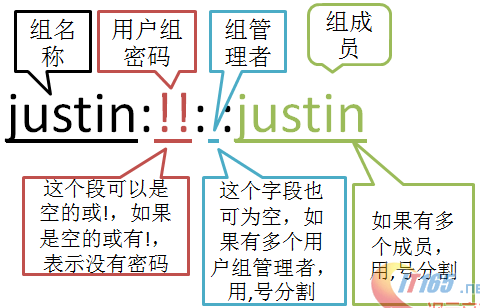
\includegraphics[width=8cm]{c2.gshadow.fields.png}
  \end{figure}
  \pause
  \vspace{-0.5cm}
  \begin{table}
    \centering
    \rowcolors[]{1}{blue!20}{blue!10}
    \begin{tabularx}{\textwidth}{clX}
      \hline
      \rowcolor{blue!50}字段 & 含义 & 说明\\
      \hline
      1 & 组名 & 用户通过它来识别组\\
      2 & 组密码 & 可以是空或\verb|!|(表示没有密码)\\
      3 & 组管理员 & 可以为空;多个组管理员用逗号隔开\\
      4 & 组成员 & 多个组成员用逗号隔开\\
      \hline
    \end{tabularx}
  \end{table}
\end{frame}

\subsection{配置文件的关系}
\begin{frame}
  \frametitle{用户和组 | 配置文件 | \alert{关系}}
  \begin{figure}
    \centering
    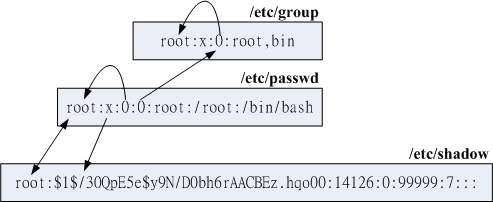
\includegraphics[width=10cm]{c2.etc.png}
  \end{figure}
\end{frame}

\section{管理账户和组}
\subsection{手动管理}
\begin{frame}
  \frametitle{用户和组 | 管理 | 手动}
  \begin{enumerate}
    \item 修改/etc/passwd:添加或删除账户行
    \item 修改/etc/shadow:添加或删除账户行
    \item 修改/etc/group:添加或删除账户引用
    \item 添加或删除账户的家目录
  \end{enumerate}
\end{frame}

\begin{frame}
  \frametitle{用户和组 | 管理 | 手动 | 添加用户}
  \begin{enumerate}
    \item 分别在/etc/passwd、/etc/group和/etc/shadow文件中添加一笔记录
    \item 创建用户家目录
    \item 在用户家目录中设置默认的配置文件
    \item 设置用户初始密码
  \end{enumerate}
\end{frame}

\subsection{命令管理}
\begin{frame}
  \frametitle{用户和组 | 管理 | \alert{命令}}
  \begin{table}
    \centering
    \rowcolors[]{1}{blue!20}{blue!10}
    \begin{tabularx}{\textwidth}{clX}
      \hline
      \rowcolor{blue!50}命令 & 说明 & 助记\\
      \hline
      \alert{useradd} & 向系统中添加账户 & Create a new user or update default new user information\\
      usermod & 修改账户属性 & Modify a user account\\
      userdel & 从系统中删除账户 & Delete a user account and related files\\
      \hline
      groupadd & 向系统中添加组 & Create a new group\\
      groupmod & 修改组的属性 & Modify a group\\
      groupdel & 从系统中删除组 & Delete a group\\
      \hline
    \end{tabularx}
  \end{table}
\end{frame}

\subsection{账户管理}
\begin{frame}[fragile]
  \frametitle{用户和组 | 管理 | 命令 | 账户管理}
  \vspace{-1em}
  \begin{table}
    \centering
    \rowcolors[]{1}{blue!20}{blue!10}
    \begin{tabular}{ccll}
      \hline
      \rowcolor{blue!50}\alert{选项} & 助记 & 说明 & 文件及字段\\
      \hline
      -c & Comment & 注释信息 & /etc/passwd,5\\
      -d & Directory & 账户的家目录 & /etc/passwd,6\\
      -e & Expire & 账号终止日期(YYYY-MM-DD) & /etc/shadow,8\\
      -f & --- & 帐号过期几日后永久停用 & /etc/shadow,7\\
      -g & Gid & 初始默认组 & /etc/passwd,4\\
      -G & Groups & 附属次要组 & /etc/group,4\\
      -m & --- & 家目录不存在时自动创建 & ---\\
      -M & --- & 强制不创建家目录 & ---\\
      -s & Shell & 默认shell & /etc/passwd,7\\
      -u & Uid & 指定用户UID & /etc/passwd,3\\
      \hline
    \end{tabular}
  \end{table}
  \pause
  \vspace{-0.5em}
\begin{lstlisting}
useradd -c COMMENT -d HOME.DIRECTORY -e EXPIRATION.DATE -f INACTIVE.DTAE -g PRIMARY.GROUP -G SECONDARY.GROUPS -m -s SHELL -u UID ACCOUNTNAME
\end{lstlisting}
\end{frame}

\begin{frame}
  \frametitle{用户和组 | 管理 | 命令 | 账户管理 | 实例}
  \begin{block}{Question}
    \begin{itemize}
      \item<2-> 账户名:unixnewbie
      \item<3-> 首要组:users
      \item<4-> 默认shell:Bourne shell
      \item<5-> 真实姓名:Jane Doe
      \item<6-> 次要组:authors
      \item<7-> 有效期:2006年7月6日
      \item<8-> 不活动天数:60天
    \end{itemize}
  \end{block}
  \begin{block}{Answer}
    \only<2>{useradd\quad -d\quad /home/unixnewbie\quad -m\quad \alert{unixnewbie}}
    \only<3>{useradd\quad -d\quad /home/unixnewbie\quad \alert{-g\quad users}\quad -m\quad unixnewbie}
    \only<4>{useradd\quad -d\quad /home/unixnewbie\quad -g\quad users\quad \alert{-s\quad /bin/sh}\quad -m\quad unixnewbie}
    \only<5>{useradd\quad \alert{-c\quad ``Jane Doe''}\quad -d\quad /home/unixnewbie\quad -g\quad users\quad -s\quad /bin/sh\quad -m\quad unixnewbie}
    \only<6>{useradd\quad -c\quad ``Jane Doe''\quad -d\quad /home/unixnewbie\quad -g\quad users\quad \alert{-G\quad authors}\quad -s\quad /bin/sh\quad -m\quad unixnewbie}
    \only<7>{useradd\quad -c\quad ``Jane Doe''\quad -d\quad /home/unixnewbie\quad \alert{-e\quad 2006-07-06}\quad -g\quad users\quad -G\quad authors\quad -s\quad /bin/sh\quad -m\quad unixnewbie}
    \only<8>{useradd\quad -c\quad ``Jane Doe''\quad -d\quad /home/unixnewbie\quad -e\quad 2006-07-06\quad \alert{-f\quad 60}\quad -g\quad users\quad -G\quad authors\quad -s\quad /bin/sh\quad -m\quad unixnewbie}
  \end{block}
\end{frame}

\begin{frame}
  \frametitle{用户和组 | 管理 | 命令 | \alert{账户管理}}
  \begin{block}{添加账户}
    创建账户:useradd\quad USERNAME\\
    创建密码:passwd\quad UERNAME
  \end{block}
  \pause
  \begin{block}{修改账户}
    修改账户名:usermod\quad -l\textcolor{gray}{(小写L)}\quad NAME.NEW\quad NAME.OLD\\
    添加到组:usermod\quad -G\quad GROUP2\quad USER\\
    修改账户属性:usermod \quad -l\quad NAME.NEW\quad -d\quad DIR\quad -g\quad GROUP\quad NAME.OLD
  \end{block}
  \pause
  \begin{block}{删除账户}
    删除账户:userdel\quad USERNAME\\
    彻底删除账户:userdel\quad -r\quad USERNAME
  \end{block}
\end{frame}

\subsection{组管理}
\begin{frame}
  \frametitle{用户和组 | 管理 | 命令 | \alert{组管理}}
  \begin{block}{添加组}
    创建组:groupadd\quad -g GID\quad GROUPNAME
  \end{block}
  \pause
  \begin{block}{修改组}
    修改组名:groupmod\quad -n\quad GROUPNAME.N\quad GROUPNAME.O\\
    修改GID:groupmod\quad -g\quad GID\quad GROUPNAME
  \end{block}
  \pause
  \begin{block}{删除组}
    删除组:groupdel\quad GROUPNAME
  \end{block}
\end{frame}

\begin{frame}
  \frametitle{用户和组 | 管理 | 命令 | 组管理 | gpasswd}
  \begin{block}{gpasswd}
    设置组密码及管理组内成员
  \end{block}
  \pause
  \begin{table}
    \centering
    \rowcolors[]{1}{blue!20}{blue!10}
    \begin{tabularx}{0.5\textwidth}{cX}
      \rowcolor{blue!50}选项 & 作用\\
      \hline
      -a & 添加用户到用户组\\
      -A & 设置用户组管理员\\
      -d & 从用户组中删除用户\\
      -M & 设置组成员列表\\
      -r & 删除用户组密码\\
      -R & 禁止用户切换为该组\\
      \hline
    \end{tabularx}
  \end{table}
\end{frame}

\subsection{实例和补充}
\begin{frame}
  \frametitle{用户和组 | 管理 | 实例}
  \begin{block}{需求}
    授权用户jack和mary对目录/software有写权限。
  \end{block}
  \pause
  \begin{block}{命令}
    \begin{enumerate}
      \item 创建新组:groupadd\quad softadm
      \item 把用户加入组:usermod\quad -G\quad softadm\quad jack;gpasswd\quad -a\quad mary\quad softadm
      \item 修改目录所属组:chgrp\quad softadm\quad /software
      \item 修改目录权限:chmod\quad g+w\quad /software
    \end{enumerate}
  \end{block}
\end{frame}

\begin{frame}
  \frametitle{用户和组 | 管理 | 补充}
  \begin{block}{禁用}
    \begin{itemize}
      \item usermod -L USERNAME
      \item passwd -l\textcolor{gray}{(小写L)} USERNAME
    \end{itemize}
  \end{block}
  \pause
  \begin{block}{恢复}
    \begin{itemize}
      \item usermod -U USERNAME
      \item passwd -u USERNAME
    \end{itemize}
  \end{block}
  \pause
  \begin{block}{删除}
    \begin{itemize}
      \item 删除用户家目录中的文件:userdel -r USERNAME
    \end{itemize}
  \end{block}
\end{frame}

\section{身份变换}
\subsection{万能的su}
\begin{frame}
  \frametitle{用户和组 | 身份变换 | su}
  \begin{table}
    \centering
    \rowcolors[]{1}{blue!20}{blue!10}
    \begin{tabular}{cl}
      \hline
      \rowcolor{blue!50}命令 & 说明\\
      \hline
      \alert{su} & Swith User\\
      \hline
      su USERNAME & 使用USERNAME账户登录\\
      su - USERNAME & 使用USERNAME的用户环境登录\\
      su & 登录到根账户\\
      \hline
    \end{tabular}
  \end{table}
\end{frame}

\begin{frame}[fragile]
  \frametitle{用户和组 | 身份变换 | su | 补充}
  \begin{block}{密码}
    \begin{itemize}
      \item 八位以上,大小写字母、数字、符号组合使用
      \item 容易记忆
      \item 定期更换
      \item 示例:\verb|Am@ri31n|
    \end{itemize}
  \end{block}
  \pause
  \begin{block}{\alert{提示符}}
    \begin{itemize}
      \item 普通用户为\verb|$|
      \item 超级用户root为\verb|#|
    \end{itemize}
  \end{block}
  \begin{figure}
    \centering
    \visible<2->{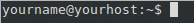
\includegraphics[width=0.45\textwidth]{c2.shell.prompt.01.jpg}}
    \visible<2->{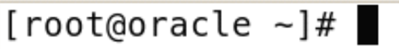
\includegraphics[width=0.45\textwidth]{c2.shell.prompt.02.png}}
  \end{figure}
\end{frame}

\subsection{安全的sudo}
\begin{frame}
  \frametitle{用户和组 | 身份变换 | sudo}
  \begin{block}{sudo (superuser do)}
    \begin{itemize}
      \item 在执行sudo命令时,临时成为root。sudo执行命令的流程是当前用户切换到root,然后以root身份执行命令,执行完成后,直接退回到当前用户。
      \item 不会泄漏root口令。使用sudo时,输入的是当前用户的密码。
      \item 仅向用户提供有限的命令使用权限。通过sudo,能把某些超级权限有针对性得下放,并且不需要普通用户知道root密码。
    \end{itemize}
  \end{block}
  \pause
  \begin{block}{sudo的用法}
    \alert{sudo\quad COMMAND}
  \end{block}
\end{frame}

\subsection{su vs. sudo}
\begin{frame}
  \frametitle{用户和组 | 身份变换 | su vs. sudo}
  \begin{block}{su的缺点}
    \begin{itemize}
      \item 不安全:su只适用于一两个人参与管理的系统,毕竟su并不能让普通用户受限得使用;超级用户root密码应该掌握在少数用户手中
      \item 麻烦:需要把root密码告知每个需要root权限的人
    \end{itemize}
  \end{block}
  \pause
  \begin{block}{sudo的特性}
    \begin{itemize}
      \item sudo:受限制的su,授权许可的su
      \item sudo能够限制用户只在某台主机上运行某些命令
      \item sudo提供了丰富的日志,详细地记录了每个用户干了什么
      \item sudo使用时间戳文件来执行类似的“检票”系统。当用户调用sudo并且输入它的密码时,用户获得了一张存活期为5分钟的票
      \item sudo的配置文件是sudoers文件(/etc/sudoers,属性为0411,编辑配置文件命令visudo),它允许系统管理员集中得管理用户的使用权限和使用的主机
    \end{itemize}
  \end{block}
\end{frame}

\begin{frame}
  \frametitle{用户和组 | 身份变换 | su vs. sudo}
  \begin{figure}
    \centering
    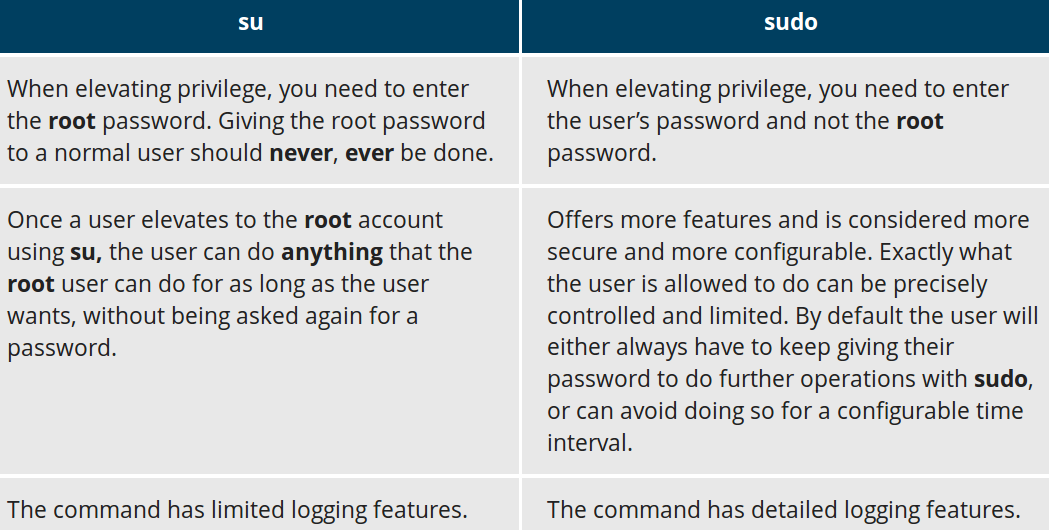
\includegraphics[width=12cm]{c2.su.sudo.png}
  \end{figure}
\end{frame}

\begin{frame}
  \frametitle{用户和组 | 身份变换 | \alert{su vs. sudo}}
  \begin{table}
    \centering
    \rowcolors[]{1}{blue!20}{blue!10}
    \begin{tabular}{cl}
      \hline
      \rowcolor{blue!50}命令 & 说明\\
      \hline
      su & 切换到root用户\\
      su - & 完全切换到root用户(环境变量,家目录都会切换过去)\\
      sudo & 普通用户执行只有管理员才能运行的命令(环境还是普通账户的)\\
      \hline
    \end{tabular}
  \end{table}
\end{frame}

\section{辅助命令}
\begin{frame}
  \frametitle{用户和组 | \alert{辅助命令}}
  \begin{table}
    \centering
    \rowcolors[]{1}{blue!20}{blue!10}
    \begin{tabular}{cl}
      \hline
      \rowcolor{blue!50}命令 & 说明\\
      \hline
      who & 列出当前在线的用户\\
      w & 显示登录的用户(进程信息)\\
      \alert{whoami} & 当前作为什么用户登录\\
      \alert{who am i} & 最初作为什么用户登录\\
      id & 显示登录的用户以及用户的组的相关信息\\
      groups & 显示用户所属的组\\
      finger & 显示用户的相关详细信息\\
      \alert{last} & 显示用户最近登录信息\\
      passwd -S & 查看用户密码状态\\
      \hline
    \end{tabular}
  \end{table}
\end{frame}

\begin{frame}
  \frametitle{用户和组 | 辅助命令}
  \begin{table}
    \centering
    \rowcolors[]{1}{blue!20}{blue!10}
    \begin{tabular}{cl}
      \hline
      \rowcolor{blue!50}命令 & 说明\\
      \hline
      newgrp & 切换用户组\\
      chgrp & 修改文件所属组\\
      chage & 更改用户密码过期信息\\
      \hline
      pwck & 检测/etc/passwd文件(锁定文件)\\
      grpck & 用户组配置文件检测\\
      vipw & 编辑/etc/passwd文件\\
      vigr & 编辑/etc/group文件(锁定文件)\\
      \hline
    \end{tabular}
  \end{table}
\end{frame}

\section{回顾与总结}
\subsection{总结}
\begin{frame}[label=current]
  \frametitle{用户和组 | 总结}
  \begin{block}{知识点}
    \begin{itemize}
      \item Linux系统中的三类账户
      \item 用户和组的配置文件
      \item 管理账户和组的常用命令
      \item 变换用户身份的方法
      \item 用户和组管理的辅助命令
    \end{itemize}
  \end{block}
  \begin{block}{技能}
    \begin{itemize}
      \item 管理用户(创建、修改、删除)
      \item 管理组(创建、修改、删除)
    \end{itemize}
  \end{block}
\end{frame}

\subsection{思考题}
\begin{frame}
  \frametitle{用户和组 | 思考题}
  \begin{enumerate}
    \item Linux系统中主要有哪三种类型的账户?
    \item 用户和组管理相关的文件主要有哪些?
    \item 解释/etc/passwd中各个字段的含义。
    \item 根据要求,使用useradd创建一个新账户。
    \item 改变用户身份的方法有哪些?
    \item 列举几个用户和组管理的辅助命令。
  \end{enumerate}
\end{frame}

\section{定制工作环境}
\begin{frame}
  \frametitle{知识拓展 | 环境变量}
  \begin{block}{环境变量}
    一个环境变量控制Linux环境的一个特定方面。\\
    环境变量将影响用户使用计算机时的视觉和感觉,以及用户可能从来不会注意到的许多底层的操作。\\
    可以使用环境变量来修改Linux环境的几乎每一个方面。
  \end{block}
  \pause
  \begin{block}{定制工作环境}
    \begin{itemize}
      \item PS1环境变量
      \item PATH环境变量
      \item 配置shell
    \end{itemize}
  \end{block}
\end{frame}

\begin{frame}
  \frametitle{知识拓展 | PS1环境变量}
  \begin{block}{PS1}
    环境变量PS1:控制命令提示符(command prompt),也就是光标前的字符串。\\
    命令提示符:用户打开一个终端窗口或者登录到控制台后,就可以看到该提示符。\\
    定制:只要使用适当的值来定义PS1环境变量,命令提示符就几乎能够包含用户所希望的任何内容。
  \end{block}
  \vspace{-1em}
  \begin{columns}
    \column{0.42\textwidth}
  \begin{figure}
    \centering
    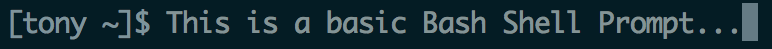
\includegraphics[width=\textwidth]{c2.prompt.01.png}\\
    \vspace{-0.2em}
    
\includegraphics[width=\textwidth]{c2.prompt.02.png}\\
    \vspace{0.2em}
    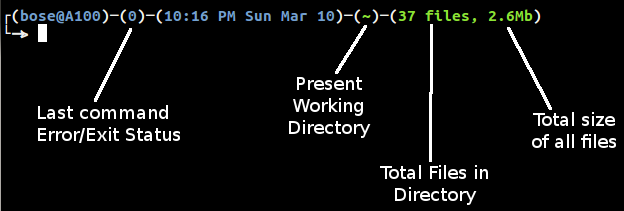
\includegraphics[width=\textwidth]{c2.prompt.03.png}\\
    \vspace{0.2em}
    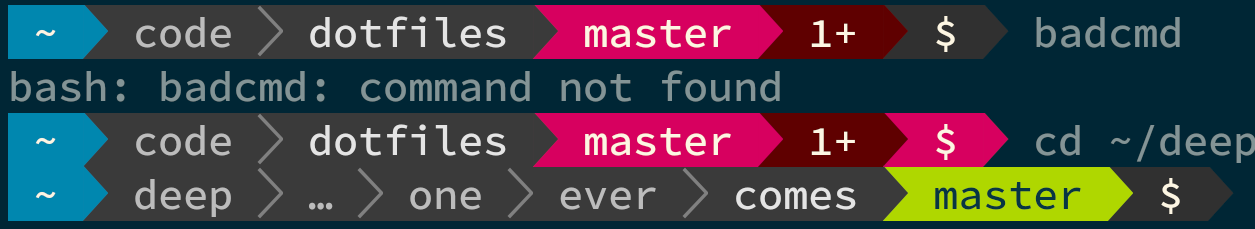
\includegraphics[width=\textwidth]{c2.prompt.04.png}\\
  \end{figure}
    \column{0.58\textwidth}
    \begin{figure}
      \centering
    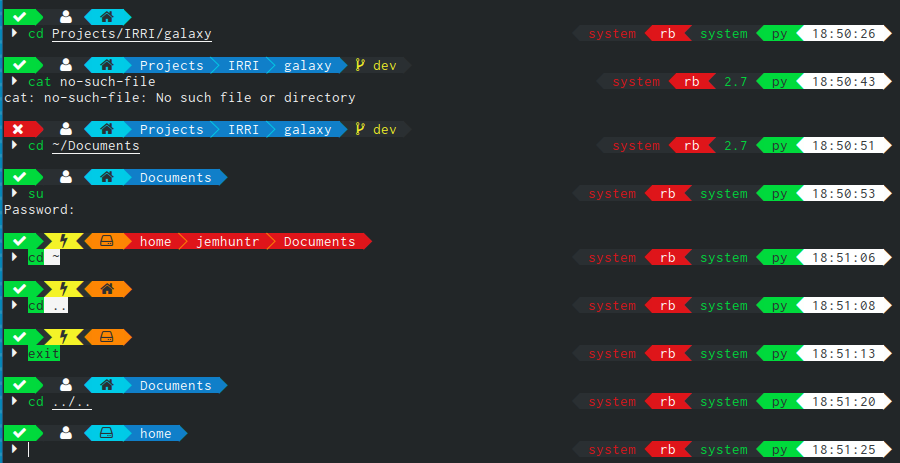
\includegraphics[width=\textwidth]{c2.prompt.05.png}
    \end{figure}
  \end{columns}
\end{frame}

\begin{frame}[fragile]
  \frametitle{知识拓展 | PS1环境变量 | 配置}
\begin{lstlisting}
PS1=">" # >
PS1="Type command here >>>" # Type command here >>>
PS1=" [\u@\h \w]\$ " # 显示用户名、主机名和工作目录
\end{lstlisting}
  \pause
  \begin{table}
    \centering
    \rowcolors[]{1}{blue!20}{blue!10}
    \begin{tabularx}{\textwidth}{cXX}
      \hline
      \rowcolor{blue!50}转义序列 & 功能\\
      \hline
      \verb|\t| & 当前时间(HH:MM:SS)\\
      \verb|\d| & 当前日期(星期、月、日)\\
      \verb|\s| & 当前的shell环境\\
      \verb|\W| & 工作目录\\
      \verb|\w| & 工作目录的绝对路径\\
      \verb|\u| & 当前用户的用户名\\
      \verb|\h| & 当前机器的主机名\\
      \verb|\$| & UID为0时使用\verb|#|,否则使用\verb|$|\\
      \hline
    \end{tabularx}
  \end{table}
\end{frame}

\begin{frame}
  \frametitle{知识拓展 | PS1环境变量 | 配置}
  \begin{block}{PS1 Generator}
    \begin{itemize}
      \item \href{http://omar.io/ps1gen/}{ps1gen}
      \item \href{https://xta.github.io/HalloweenBash/}{Bash Profile Generator}
      \item \href{http://bashrcgenerator.com/}{.bashrc generator}
      \item \href{http://ezprompt.net/}{Easy Bash PS1 Generator}
      \item \href{https://www.kirsle.net/wizards/ps1.html}{Bash \$PS1 Generator 2.0}
      \item \href{https://www.askapache.com/linux/bash-power-prompt/}{Crazy POWERFUL Bash Prompt}
    \end{itemize}
  \end{block}
\end{frame}

\begin{frame}[fragile]
  \frametitle{知识拓展 | PATH环境变量}
  \vspace{-0.5em}
  \begin{block}{PATH环境变量}
    \begin{itemize}
      \item PATH环境变量包含一组目录,可执行程序可能位于这些目录中。
      \item 如果PATH变量的值中含有某个目录,那么调用该目录中的可执行文件时就不需要输入目录名。
      \item PATH变量的值通常在一个配置文件中设置,具有全局意义。
      \item 用户可以向PATH变量中添加自己的值。
      \item 尽管大多数用户不需要考虑将目录名添加到PATH值中的次序,但有些时候这个次序是很重要的。
      \item shell依次在PATH目录中查找命令,只要发现匹配的程序,就会启动改程序。
    \end{itemize}
  \end{block}
  \pause
  \vspace{-1em}
\begin{lstlisting}
PATH=$PATH:NewPath # 向PATH变量添加值的格式
PATH=$PATH:/home/joe/bin
# 一次添加多个目录,用冒号将这些目录隔开
PATH=$PATH:/home/joe/bin:/home/joe/myprog/bin
\end{lstlisting}
\end{frame}

\begin{frame}
  \frametitle{知识拓展 | 配置shell}
  \begin{block}{shell启动与运行控制文件}
    \begin{itemize}
      \item 当shell启动时,它解析所有可用的运行控制文件。
      \item shell检查的第一个运行控制文件是一个/系列全局配置文件。
      \item 完成全局配置文件的解析之后,shell接着解析存储在用户账户中的任何已有的个人配置文件。
    \end{itemize}
  \end{block}
  \pause
  \begin{block}{shell会话类型}
    \begin{itemize}
      \item 确切的启动顺序依赖于要运行的shell会话类型。
      \item 有两种shell会话类型
        \begin{itemize}
          \item 登录shell会话:提示用户输入用户名和密码
          \item 非登录shell会话:在GUI下启动终端会话时出现
        \end{itemize}
    \end{itemize}
  \end{block}
\end{frame}

\begin{frame}
  \frametitle{知识拓展 | 配置shell | 启动顺序}
  \begin{block}{登录shell会话}
  \begin{table}
    \centering
    \rowcolors[]{1}{blue!20}{blue!10}
    \begin{tabularx}{\textwidth}{ccX}
      \hline
      \rowcolor{blue!50}顺序 & 配置文件 & 文件用途\\
      \hline
      1 & \verb|/etc/profile| & 应用于所有用户的全局配置脚本\\
      2 & \verb|~/.bash_profile| & 用户个人的启动文件;可以用来扩展或重写全局配置脚本中的设置\\
      3 & \verb|~/.bash_login| & 如果文件2没有找到,bash会尝试读取这个脚本\\
      4 & \alert{\verb|~/.profile|} & 如果文件2或3都没有找到,bash会试图读取这个文件\\
      \hline
    \end{tabularx}
  \end{table}
  \vspace{-1em}
  \end{block}
  \pause
  \begin{block}{非登录shell会话}
  \begin{table}
    \centering
    \rowcolors[]{1}{blue!20}{blue!10}
    \begin{tabularx}{\textwidth}{ccX}
      \hline
      \rowcolor{blue!50}顺序 & 配置文件 & 文件用途\\
      \hline
      1 & \verb|/etc/bash.bashrc| & 应用于所有用户的全局配置文件\\
      2 & \alert{\verb|~/.bashrc|} & 用户个人的启动文件;可以用来扩展或重写全局配置脚本中的设置\\
      \hline
    \end{tabularx}
  \end{table}
  \end{block}
\end{frame}

\begin{frame}[fragile]
  \frametitle{知识拓展 | 配置shell | $\sim$/.profile}
\begin{lstlisting}
# .bash_profile
# Get the aliases and functions
if [ -f ~/.bashrc ]; then
  . ~/.bashrc
fi

# User specific environment and startup programs
PATH=$PATH:$HOME/bin
export PATH
\end{lstlisting}
\end{frame}

\begin{frame}[fragile]
  \frametitle{知识拓展 | 配置shell | $\sim$/.bashrc}
\begin{lstlisting}
umask 0002
export HISTSIZE=1000
alias ll='ls -l --color=auto'

case "$TERM" in
xterm-color)
    PS1='[${debian_chroot:+($debian_chroot)}\[\033[01;32m\]\h\[\033[00m\]] \[\033[01;34m\]\w\[\033[00m\]\$ '
    ;;
*)
    PS1='[${debian_chroot:+($debian_chroot)}\h] \w\$ '
    ;;
esac
\end{lstlisting}
\end{frame}

\begin{frame}
  \frametitle{下节预告}
  \begin{itemize}
    \item 安装Windows系统时的分区过程
    \item Windows系统的目录结构、路径写法
    \item 日常使用中基本的目录和文件操作
    \item Windows系统中的快捷方式
  \end{itemize}
\end{frame}


\section*{Acknowledgements}
\begin{frame}
  \frametitle{Powered by}
  \begin{center}
    
\includegraphics[width=9cm]{power.png}
  \end{center}
\end{frame}

\end{document}

